\chapter{Results and discussion}\label{chap:Results&Disc}

\section{Biochar analyses and characterization}

\subsection{Biochar properties}
Table of pyrolysis yield, ash content, energies etc. 

\subsection{Enrichment factor}
Calculation of enrichment factor for C – potential for carbon storage
mention ETIA measurements

\section{Biochar properties}

\subsection{Iron and copper speciation}
Synchrotron

\subsection{Surface area and pore volume}
N2/CO2 sorptometry
Pore size distribution

\begin{table}
\centering
\caption{Surface area and pore volume determined by BET and DFT theories, respectively. $\mathrm{CO_2}$ represents pores 0.4-1.5 nm, $\mathrm{N_2}$ represents pores \textgreater 1.5 nm.}
\label{tab:SAPV}
\begin{tabular}{lccc|cc}
\toprule
              &   & \multicolumn{2}{c}{\textbf{N\textsubscript{2}}} & \multicolumn{2}{c}{\textbf{CO\textsubscript{2}}} \\  \cline{3-6} \addlinespace
              &  & BET-SA         & BJH-PV         & DFT-SA          & DFT-PV         \\ \midrule
\textbf{Sample} & \textbf{PT (\textdegree C)} & $\mathrm{m^2/g}$  & cc/g           & $\mathrm{m^2/g}$            & cc/g           \\ \midrule
ULS         & 700                    & 128.31         & 0.126          & 164.58          & 0.047          \\
CWC         & 700                    & 323.33         & 0.017          & 683.27          & 0.186          \\
DSL         & 700                    & 110.14         & 0.111          & 86.55           & 0.027         \\ \midrule
\end{tabular}
\end{table}



\begin{table}
\caption{Effective cross-sectional diameter (D\textsubscript{eff}) and maximum diameter (D\textsubscript{max}) of TCs interpolated and extrapolated by linear regression from calculations performed by \citep{inoue2012size} on PFOA and other PFCAs with chain lengths 11-18.}
\centering
\begin{threeparttable}
\label{tab:molecsize}
\begin{tabular}{lccc}
\toprule
Compound & \begin{tabular}[c]{@{}c@{}}Carbon chain \\ length\end{tabular} & \begin{tabular}[c]{@{}c@{}}D\textsubscript{eff} \\ (nm)\end{tabular} & \begin{tabular}[c]{@{}c@{}}D\textsubscript{max} \\ (nm)\end{tabular} \\ \midrule
PFPeA    & 5                                                              & 0.45                                                 & 0.96                                                 \\
PFHxA    & 6                                                              & 0.50                                                 & 1.08                                                 \\
PFHpA    & 7                                                              & 0.56                                                 & 1.19                                                 \\
PFOA\textsuperscript{*}     & 8                                                              & 0.61                                                 & 1.36                                                 \\
PFNA     & 9                                                              & 0.67                                                 & 1.42                                                 \\
PFDA     & 10                                                             & 0.72                                                 & 1.54  \\ \bottomrule                                    
\end{tabular}
\begin{tablenotes}
\item \textsubscript{*} Calculated value from \citep{inoue2012size}
\end{tablenotes}
\end{threeparttable}
\end{table}

\subsection{Total elemental composition}


\begin{table}
\centering
\caption{Total element composition of the biochars used in this thesis.}
\adjustbox{max width=\textwidth}{
\label{tab:totelem}
\begin{tabular}{llccccccc} 
\toprule
\textbf{}               & \textbf{}      & \textbf{} & \multicolumn{2}{c}{\textbf{CWC}} & \multicolumn{2}{c}{\textbf{ULS}} & \multicolumn{2}{c}{\textbf{DSL}} \\ \cline{4-9} 
                        &                &           & Mean              & Std.dev          & Mean             & Std.dev           & Mean            & Std.dev            \\ \hline \addlinespace
Pyrolysis temperature   &                &           & 700               &                  & 700              &                   & 700             &                    \\
pH                      & 1:5 in water   & -         & 9.6               & 0.1              &                  &                   & 9.68            &                    \\
Conductivity            & 1:5 in water   & µS/cm     & 1268              & 263              &                  &                   &                 &                     \\ \addlinespace \hline
\textbf{Main elements}  & \textbf{}      &           &                   &                  &                  &                   &                 &                    \\ \hline \addlinespace
C                       &                & \%        & 91.4              & 2.5              & 29.63            & 0.47              & 13.5            & 0.2                \\
N                       &                & \%        & 0.69              & 0.02             & 1.131            & 0.039             & 0.82            & 0.02               \\
H                       &                & \%        & 1.01              & 0.14             & 1.243            & 0.045             & 1.05            & 0.16               \\
O                       & Calculated     & \%        &                   &                  &                  &                   &                 &                    \\
Ca                      & $\mathrm{HNO_3}$ digestion & g/kg      & 8.0               & 0.2              & 21               &                   & 26.0            & 0.0                \\
Fe                      & $\mathrm{HNO_3}$ digestion & g/kg      & 0.13              & 0.04             & 23               &                   & 180             & 0                  \\
K                       & $\mathrm{HNO_3}$ digestion & g/kg      & 4.03              & 0.06             & 6.8              &                   & 3.7             & 0.1                \\
Mg                      & $\mathrm{HNO_3}$ digestion & g/kg      & 0.91              & 0.02             & 5.3              &                   & 4.70            & 0.17               \\
Na                      & $\mathrm{HNO_3}$ digestion & g/kg      & 0.05              & 0.00             & 2.4              &                   & 1.83            & 0.06               \\
P                       & $\mathrm{HNO_3}$ digestion & g/kg      & 0.41              & 0.01             & 45               &                   & 8.0             & 0.5                \\
S                       & $\mathrm{HNO_3}$ digestion & g/kg      & 0.09              & 0.00             & 2.9              &                   & 7.23            & 0.68               \\
Si                      & $\mathrm{HNO_3}$ digestion & g/kg      & 0.17              & 0.02             & 1.7              &                   & 0.62            & 0.08               \\ \addlinespace \hline
\textbf{Trace elements} & \textbf{}      &           &                   &                  &                  &                   &                 &                    \\ \hline \addlinespace
As                      & $\mathrm{HNO_3}$ digestion & mg/kg     & 0.01              & 0.00             & 3.0              &                   & 3.13            & 0.21               \\
Ba                      & $\mathrm{HNO_3}$ digestion & mg/kg     & 216.67            & 5.77             & 310              &                   & 177             & 6                  \\
Cd                      & $\mathrm{HNO_3}$ digestion & mg/kg     & 0.00044           & -                & 0.0081           &                   & 0.03            & 0.00               \\
Co                      & $\mathrm{HNO_3}$ digestion & mg/kg     & 0.30              & 0.03             & 7.1              &                   & 9.97            & 0.06               \\
Cr                      & $\mathrm{HNO_3}$ digestion & mg/kg     & 1.69              & 1.22             & 56               &                   & 53.3            & 1.5                \\
Cu                      & $\mathrm{HNO_3}$ digestion & mg/kg     & 5.17              & 0.60             & 220              &                   & 277             & 6                  \\
Mo                      & $\mathrm{HNO_3}$ digestion & mg/kg     & 0.06              & 0.02             & 7.1              &                   & 19.0            & 0.0                \\
Ni                      & $\mathrm{HNO_3}$ digestion & mg/kg     & 1.77              & 0.64             & 41               &                   & 34.7            & 0.6                \\
Pb                      & $\mathrm{HNO_3}$ digestion & mg/kg     & 0.08              & 0.02             & 13               &                   & 25.3            & 4.0                \\
Sr                      & $\mathrm{HNO_3}$ digestion & mg/kg     & 36                & 2                & 87               &                   & 120             & 0                  \\
V                       & $\mathrm{HNO_3}$ digestion & mg/kg     & 0.10              & 0.02             & 34               &                   & 54.0            & 1.0                \\
Zn                      & $\mathrm{HNO_3}$ digestion & mg/kg     & 3.2               & 0.6              & 480              &                   & 0.80            & 0.01      \\ \bottomrule        
\end{tabular}}
\end{table}

\subsubsection{C/O and C/H ratios}

\subsection{PZC}

\section{Soil chemistry}
The soil used in the batch tests was characterized as a fine sand (0.1 to 0.3 mm) with 1.3 \% TOC (pH 5.38 \textpm 0.02 , CEC 2.63 \textpm 0.06 meqv 100 g\textsuperscript{-1}). Total element concentrations and exchangeable ion concentrations are in \ref{appSec:misclab}. 

PFAS contamination?



\section{pH and conductivity}
pH varied little between all biochar-soil-water systems with an average pH of 7.18 \textpm 0.02. Conductivity was 39 \textpm 0.9 \textmu S cm\textsuperscript{-1}. Since the variance is low, pH and conductivity will not be considered as factors that influence sorption of PFCAs. whereby conductivity of soil-water samples differed the most from the rest of the samples with a mean conductivity of 23 \textpm 0.05 \textmu S cm\textsuperscript{-1} versus a mean of 41 \textpm 0.9 \textmu S cm\textsuperscript{-1} for the biochar-water and biochar-soil-water samples. Complete pH and conductivity data is in \cref{appSec:misclab} 

\begin{table}
\centering
\caption{Mean and standard deviation of pH and conductivity (\textmu S/cm) measurements for the different batch test systems (n=3). BC:S:H\textsubscript{2}O is the biochar:soil:water ratio.}
\label{tab:pHcond}
\begin{tabular}{lccccc}
\toprule
 & \multicolumn{2}{c}{pH} & \multicolumn{2}{c}{Conductivity} & \\
 & mean & std. dev & mean & std. dev & BC:S:H20\\
\midrule
ULS & 7.10 & 0.04 & 45.70 & 3.03 & 1:0:500\\
DSL & 7.31 & 0.02 & 40.93 & 1.07 & 1:0:500\\
CWC & 7.36 & 0.07 & 46.47 & 0.70 & 1:0:500\\
ULS+S & 7.18 & 0.02 & 34.93 & 0.40 & 1:50:500\\
DSL+S & 7.14 & 0.00 & 35.73 & 1.50 & 1:50:500\\
CWC+S & 7.09 & 0.05 & 44.90 & 1.54 & 1:50:500\\
S & 7.08 & 0.05 & 23.33 & 0.87 & 0:1:10\\
\bottomrule
\end{tabular}
\end{table}

\subsection{PFAS-contamination}

\begin{table}[htb]
\centering
\caption{Total concentration (mg/kg dw), exchangeable ions (meqv/100 g) and summary parameters for the soil used in the batch leaching tests.}
\label{tab:soil}
\begin{tabular}{llll} \toprule
\multicolumn{2}{c}{\textbf{Total concentration}} & \multicolumn{2}{c}{\textbf{Exchangeable ions}} \\ \hline \addlinespace
Ba                       & 11.0 ± 0.3                       & Al\textsuperscript{3+}                              & 0.87 ± 0.01              \\
Be                       & 0.27 ± 0.004                        & H\textsuperscript{+}                               & 0.088 ± 0.03              \\
Cd                       & 0.20 ±0.06                        & Mg\textsuperscript{2+}                              & 0.07 ± 0.001               \\
Co                       & 2.07 ± 0.09                         & Ca\textsuperscript{2+}                              & 1.54 ± 0.03              \\
Cr                       & 6.13 ± 0.4                        & Na\textsuperscript{+}                                 & 0.009 ± 00004                  \\
Cu                       & 9.10 ± 1                        & K\textsuperscript{+}                                 & 0.046 ± 0.0002                  \\
Fe                       & 6740 ± 445                     &                                   &                          \\
Hg                       & \textless{}1                       &                                   &                          \\
Mn                       & 124 ± 7                      & \multicolumn{2}{c}{\textbf{Summary parameters}}              \\  \cline{3-4} \addlinespace
Ni                       & 3.09 ± 0.2                        & CEC                               & 2.62 ± 0.07              \\
P                        & 525 ± 29                      & pH (H\textsubscript{2}O)                          & 5.38 ± 0.02              \\
Pb                       & 8.45 ± 0.5                         & pH (0.01 M CaCl\textsubscript{2})                 & 4.36 ± 0.01               \\
Sr                       & 6.80 ± 0.7                          & Conductivity (\textmu S/cm)              & 23 ± 0.9                \\
V                        & 12.67 ± 0.9                       & C-org (\%)                        & 1.32 ± 0.03              \\
Zn                       & 22.20 ± 1                           & N-tot (\%)                        & 0.11 ± 0.003 \\ \bottomrule             
\end{tabular}
\end{table}

\section{Sorption of PFAS: single-compound isotherms BC-water}

\begin{figure}
    \centering
    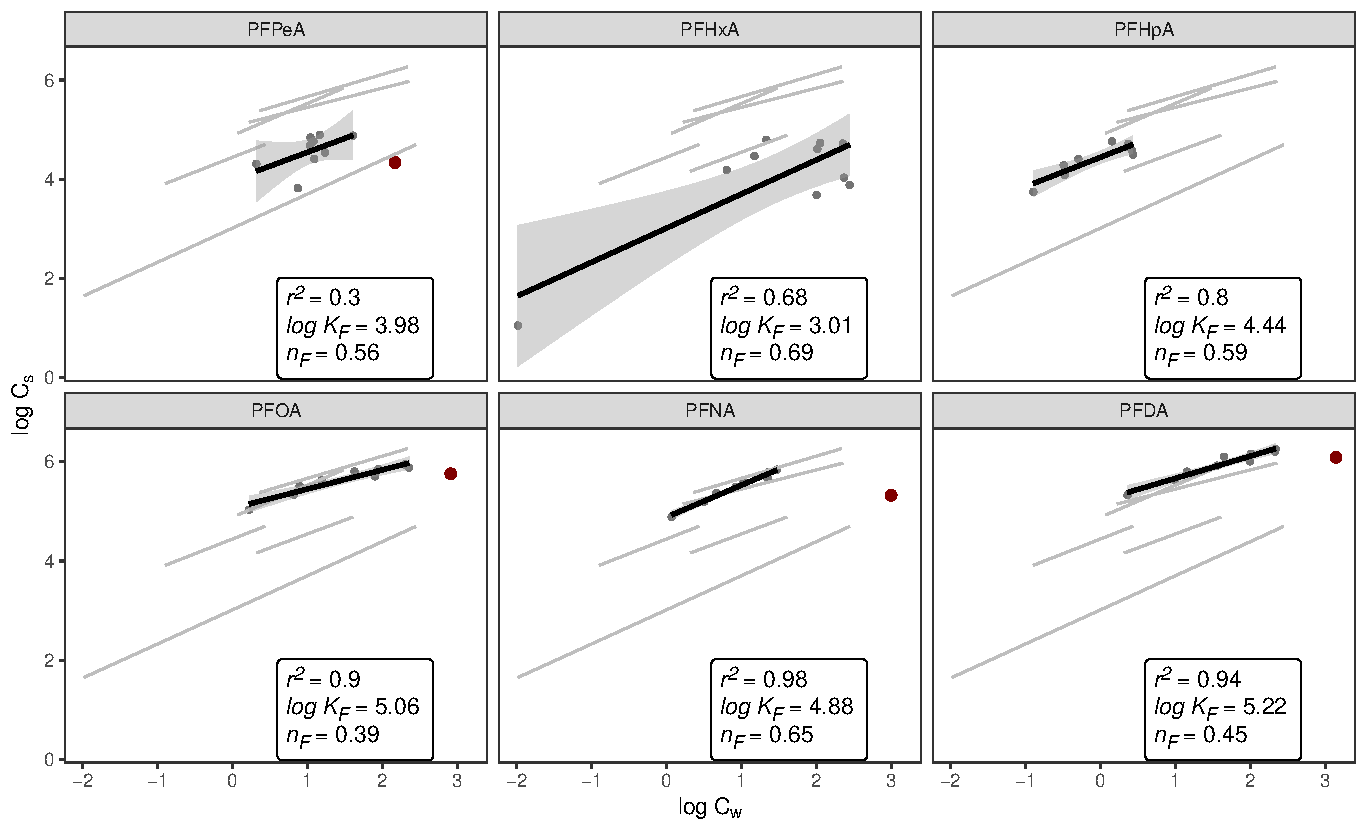
\includegraphics[width=\textwidth]{R/figs/CWC_facet_isotherm.pdf}
    \caption{CWC isotherm}
    \label{fig:CWC_isotherm}
\end{figure}

\begin{figure}
    \centering
    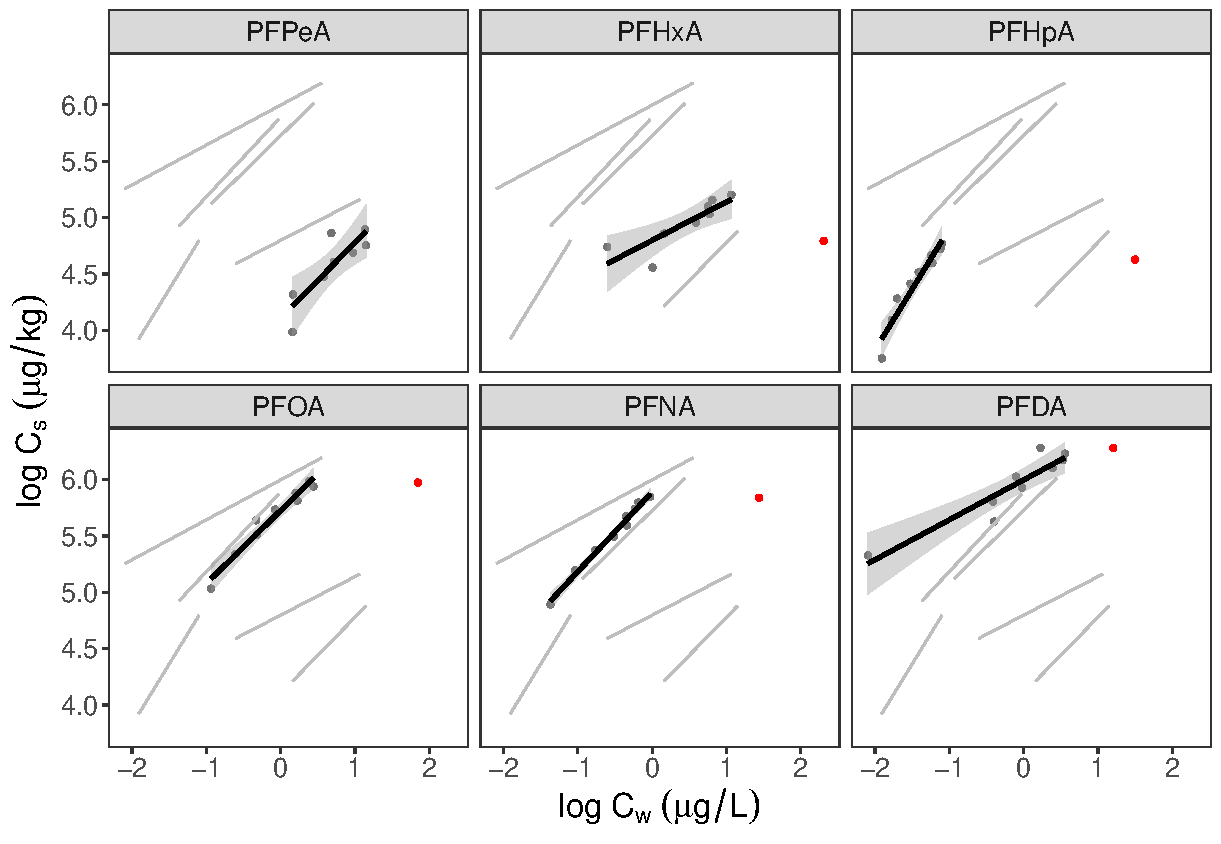
\includegraphics[width=\textwidth]{R/figs/ULS_facet_isotherm.pdf}
    \caption{ULS isotherm}
    \label{fig:ULS_isotherm}
\end{figure}

\begin{figure}
    \centering
    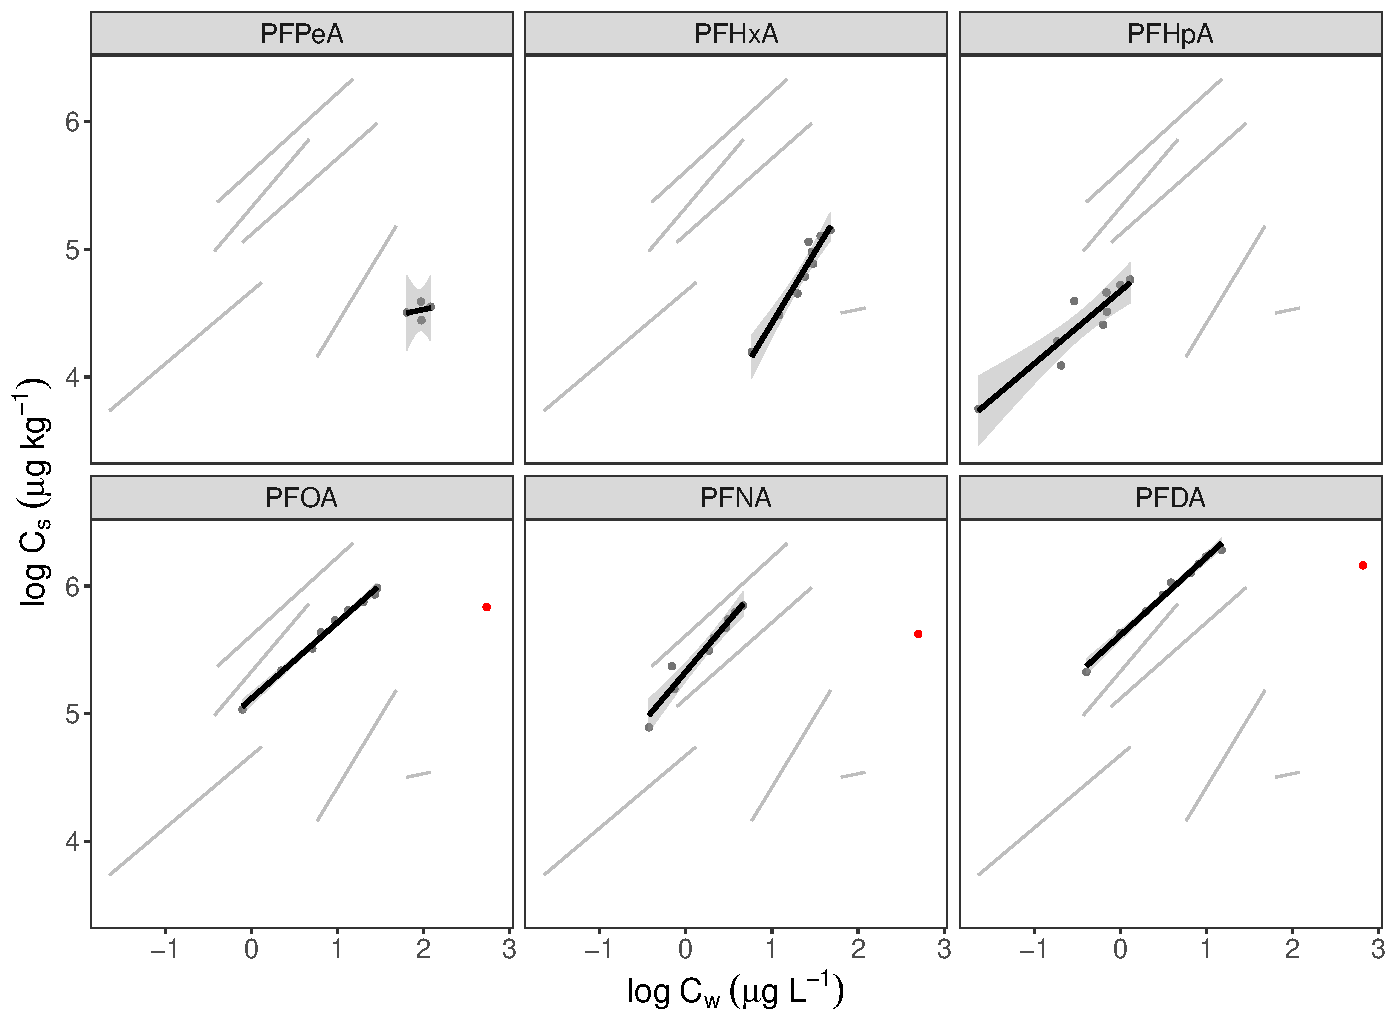
\includegraphics[width=\textwidth]{R/figs/DSL_facet_isotherm.pdf}
    \caption{DSL isotherm}
    \label{fig:DSL_isotherm}
\end{figure}
Table with partitioning coefficients for the biochar sorbents with and without the presence of soil, plus/minus standard deviation
\subsubsection{Freundlich parameters}
Meaning of parameters KF and n
Importance of nonlinearity and concentration interval achieved 
Comparison of KF across concentration magnitudes, conversion factor and why

\subsubsection{Biochar sorbent properties vs sorption}
Correlation plots:
    Iron speciation vs KF
    Surface area vs KF 
    Pore volume vs KF 
    C:O vs KF 
    C:H vs KF  
Discussion on how these factors influence sorption, sorption capacity and sorption affinity of biochars

\subsubsection{Sorption mechanisms}

\subsubsection{Influence of PFAS chain length}

\begin{figure}
    \centering
    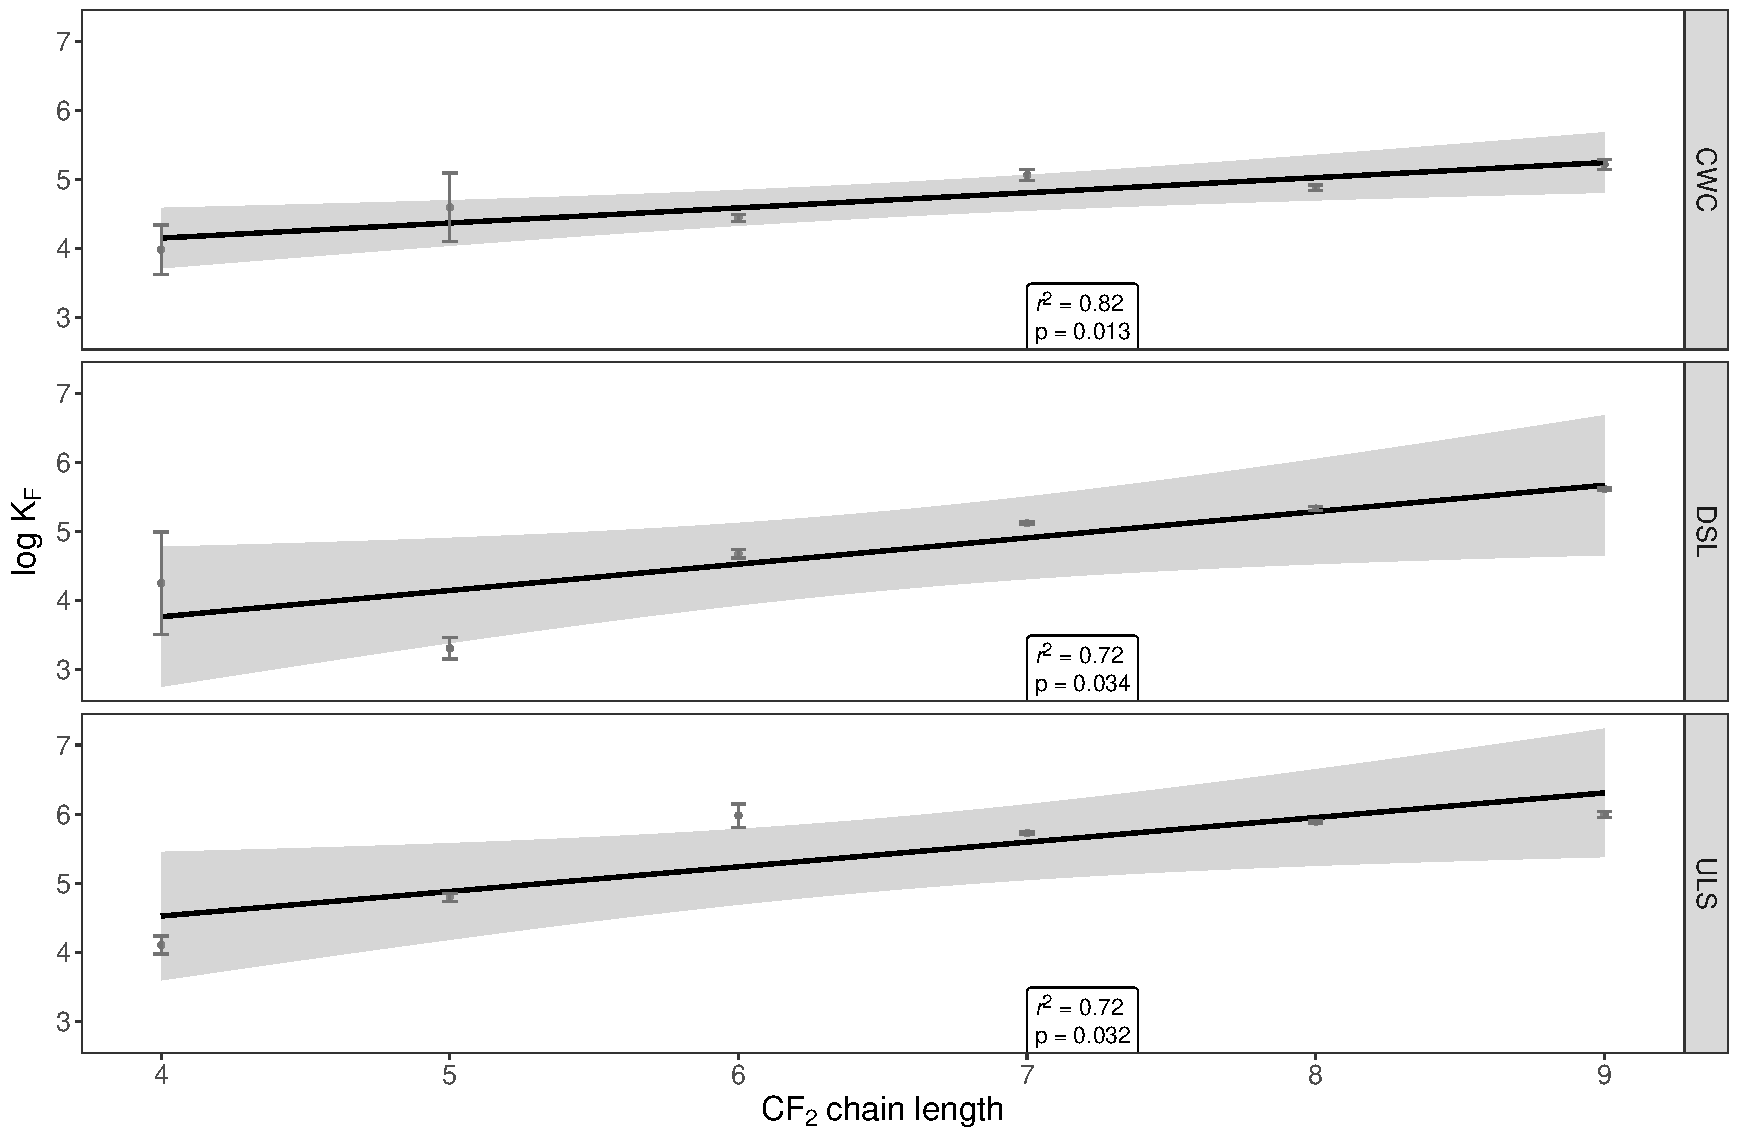
\includegraphics[width=\textwidth]{R/figs/chainlength_KF.pdf}
    \caption{Correlation plot of $log K_F$ as a function of PFCA chain length (number of $CF_2$ moieties) for the different biochars fitted by a linear model. The error bars represent the standard deviation of $log K_F$ (n=9).}
    \label{fig:chainlength}
\end{figure}
 
Discuss reasons based on correlation plots
    hydrophobic effect, congeners comparison
    size exclusion (find molecular size?)
    Biochar properties
        C/H, C/O ratio, degree of condensation
        Porosity, surface area

\subsubsection{Influence of PFAS functional group}
Biochar properties
    Point of zero charge
    Surface functional groups, charge
    Iron content, charge
    Electrostatic interaction

\section{Biochar PFAS sorption efficiency: cocktail isotherms BC-water}
Biochar removal efficiency 
Freundlich parameters
Attenuation factors

\section{Biochar PFAS sorption efficiency: single-compound isotherms BC-soil-water}
Kd at C10 for soil alone
How to account for Kd of soil when calculating KF 
    Show how to derive Freundlich equation with respect to soil Kd from original Freundlich equation
    
\subsection{PFOA isotherms vs cocktail isotherms}
to compare with C$_w$ at SP10 for the single compound batch test to determine a competition factor between the other PFCAs in the cocktail to sorption sites on the biochar.

Plot comparing the isotherms of PFOA-BC to PFOA-soil-BC
Discuss influence of presence of soil on PFOA sorption
Significance of C8 chain length taken together with BC properties 

Plot comparing cocktail-BC to cocktail-soil-BC
Effect of presence of soil AND competing congeners
Competitive sorption, attenuation factor

Comparison between sorption of PFOA in cocktail-soil and PFOA in biochar-soil

\subsection{Sorption attenuation by soil}
fouling/pre-loading by NOM
Pore blocking

\subsection{Soil-BC interactions}

\subsubsection{Soil contamination}

\subsubsection{Difference in color of filtrate between batch tests}
Filter clogging and reduction in filter size, had to exchange filters during filtration, how this may impact results
Aggregation of humic substances upon addition of acetic acid pre-SPE, how this may impact results

Precipitation of a brown fluff was observed when filtered batch tests containing soil was adjusted to pH 3 with 1 M acetic acid

\begin{figure}
    \centering
    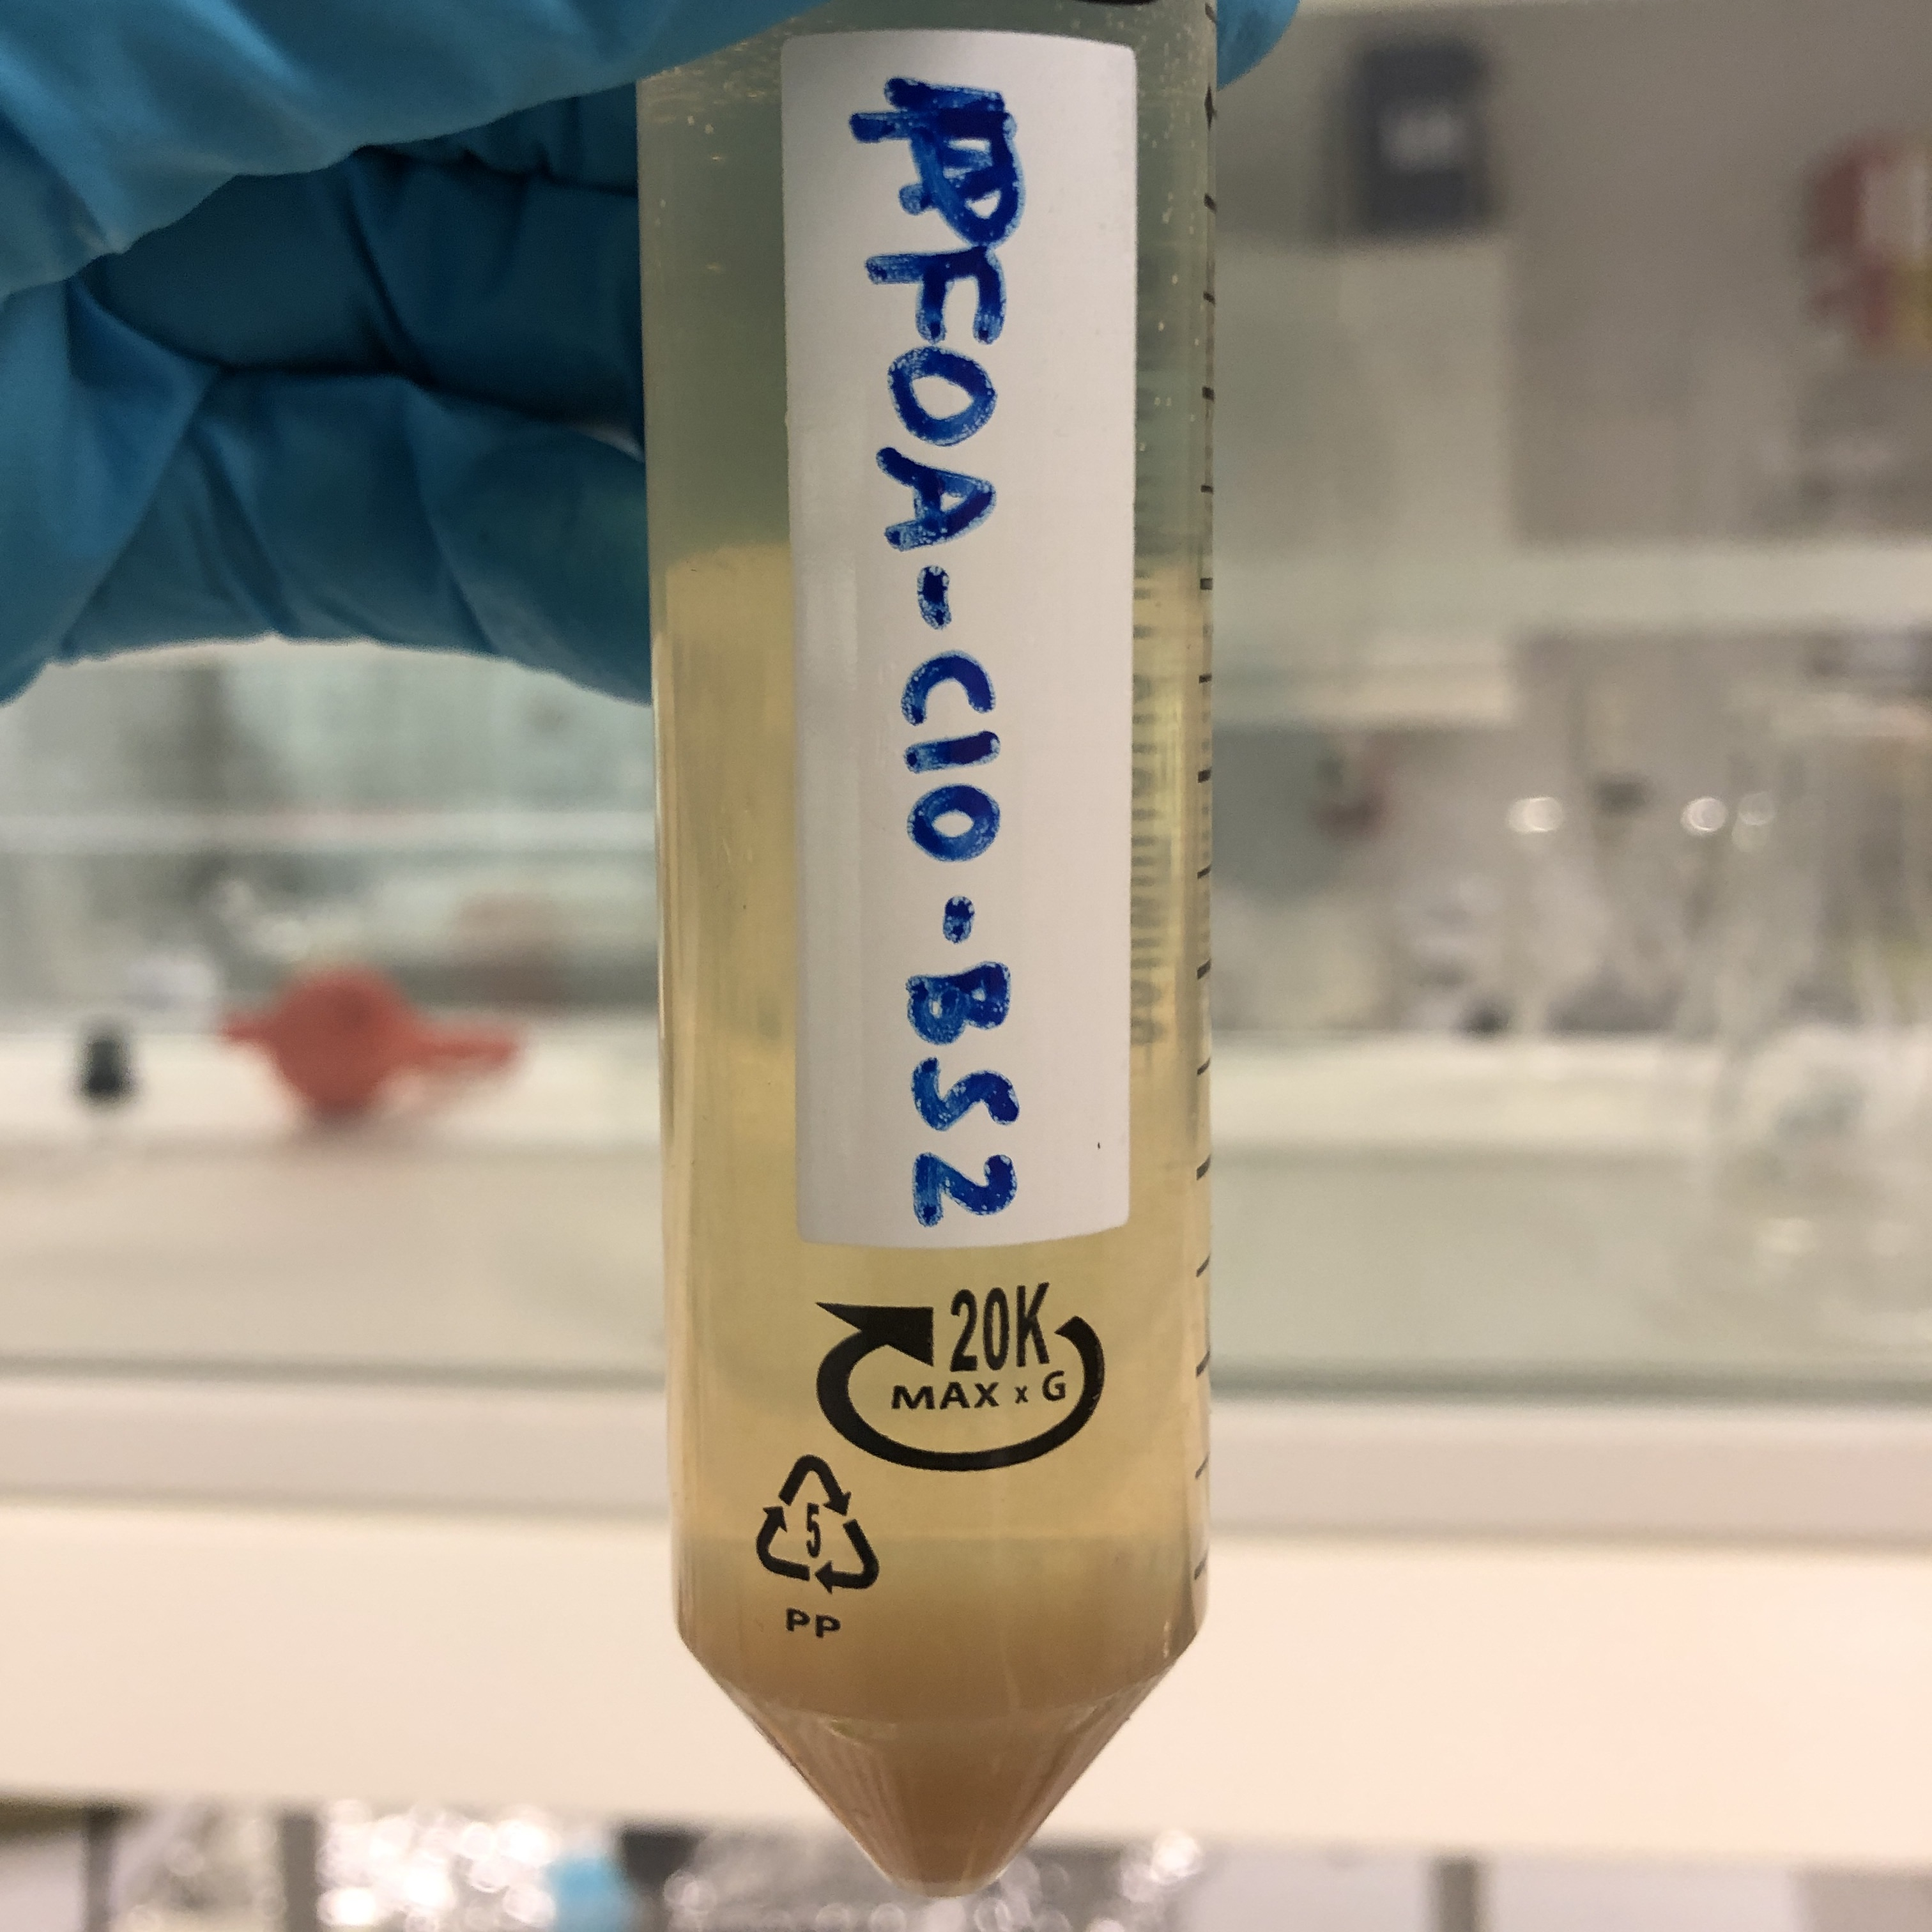
\includegraphics[width=0.6\linewidth,scale=0.6]{Bilder/Samples/Precipitation.jpg}
    \caption{Precipitation observed when filtered soil samples were adjusted to pH 3 with 1 M acetic acid.}
    \label{fig:precip}
\end{figure}

\section{Potential for commercializing sludge chars as sorbents}
\subsection{Sorbent quality}
Removal efficiency, good enough for application?
\subsubsection{EBC limits heavy metals}
Leaching of heavy metals results at PT 700 C
    As, Cd, Co, Zn, Pb for all chars Below EBC limits, Cr and Ni between lower and upper limit
    EBC = European Biochar Certificate
    Cu above EBC limits for ULS and DSL
    Enrichment factors heavy metals (?)

\subsubsection{Field conditions representativeness}
Soil pH, sorption/desorption of PFAS
Protonation state of PFAS (pKa) unaffected at environmentally relevant pH’s
Leaching in acid soil not a problem, will increase sorption affinity of charged carboxyl to protonated BC surface
Alkaline conditions, liming?? 
    Depends on the dominating sorption mechanism
    Repulsion: functional groups, iron oxides, changes charge with pH?
    If hydrophobic interactions are dominating, sorption will likely not be affected
Equilibrium conditions vs laboratory batch tests
BC dose

Are the results representative of what goes on in real life? Sorption by shaking for 14 days represent an assumed equilibrium between PFCAs in the water and soil phase. A comparable situation in the field would be washing of the soil with large amounts of water such as during heavy rainfall. This will only be the case during occasional stormwater events and thus the results from this research could benefit from being supplemented with results from leaching tests using biochar mixed with soil. However, the relationship:

\begin{align}
    \frac{k_1}{k_2}
\end{align}

where \(k_1\) is the PFCA sorption (adsorption and absorption) rate and \(k_2\) is the PFCA desorption rate, where \(k_1>>k_2\), which indicates that sorption is many times higher, and in an equilibrium situation, sorption and desorption will be at steady state \citep{Cornelissen2005}. 


\section{Sustainability}
\subsection{Pyrolysis energy demand}
\subsection{Life cycle impact assessment (LCIA)}
LCA (life cycle assessment), sustainability aspects of production of biochar
High operating energy and cost different technologies \citep{Alhashimi2017}

\section{Quality control of laboratory analysis and uncertainty}

\subsection{Spiking standard concentrations}
SPE and directly, why?

The pipettes used for making the PFCA dilutions were calibrated. The three pipettes were: 1) 2-10 mL, 2) 200-1000 \textmu L, and 3) 5-50 \textmu L. All pipettes were below the permitted coefficient of variation (CV = 0.3, 0.5, and 2 $\%$ respectively (\cref{appSec:misclab}, \crefrange{appTab:pip2-10}{appTab:pip5-50}).

Since the diameter of the centrifuge tube (30 mm) was larger than that of a volumetric flask and biochar was added prior to the dilution process, the final concentration of the sorbent-sorbate mixture may have a heightened inaccuracy. However, the volume of which 0.1 g biochar occupies can be considered insignificant due to the high absorptive capacity of biochar and small mass used. Therefore a set of 10 centrifuge tubes filled to 50 mL containing 0.1 g CWC were weighed to control the uncertainty of the final dilutions. The results from weighing show that the weight of 10 trials were not accurate but precise, which means that all samples were prepared with the same final volume even though this volume deviates from 50 mL (\cref{appTab:PPcentrifuge}). 

Volume 50 mL weighed vs by eye measurement, diameter of test tube and error
preparation of cocktail standard, not consistent, some individual pipetting. 

\subsubsection{Filter blanks no significant difference}

\subsection{PFAS losses during laboratory analysis}
SPE protocol, many steps, many PP test tubes transfers, saturated PFAS-solutions, internal standard (dilutions had to disregard IS because too low concentration)

\citep{Lath2019labsorb}: 
Syringe filters: sorption of PFOA to centrifuge tubes and filter membranes. Sorption onto syringe surface: negligible due to short residence time (\textless 10 s). 74\% recovery from regenerated cellulose syringe filter. No improvement in recovery was seen when conditioning the syringe filters with phosphate solution or methanol. No trend between losses of PFOA on syringe filter and increasing spike concentrations. Centrifugation only is therefore advised if possible to avoid filtration losses. 

Test tubes: Greater recoveries from glass tubes than plastic, PP poorest recovery (55-68 \% recovery)... Contact time of PFAS residing in tubes for longer than 7 days should not be of significance, as \citep{Lath2019labsorb} propose that sorption and saturation of tube walls occur within hours. 74-81 \% recovery for PP when testing dependence on pH and ionic strength. Slight pH dependence, higher recovery at higher pH due to repulsion of negatively charged functional groups (PP has negative surface charge above pH 3.5-4. Bridging effect will be observed at higher pH's between cations like Ca2+, but is still considered negligible compared to the losses due to the physicochemical properties of the materials themselves. In general PP and plastics consists of mainly carbon hydrogen chains and are more hydrophobic than glassware. Sorption to tube walls saturate, so recoveries increase significantly with higher spike concentrations (e.g. for PP, 12-415 ug/L spiked PFOA increased recovery from 53.7-85.5 \%). Therefore, quantification of low concentrations may be subject to highest error, and in most cases will be an underestimation of dissolved concentrations. 

Use of PP test tubes, study
Higher probability of underestimating Cw for low-concentration samples because tube walls saturate – maximum number of sorption sites, there is a sorption maximum (Langmuir)

\subsection{Uncertainty}
\subsubsection{Batch tests}
Vel, du kan jo prøve å legge sammen alle de feilene. Det finnes jo forskjellige typer feilkilder i et stort forsøksoppsett. Det man ofte ser er at det er en eller to feil som er så store at de overskygger de andre. Da er det ikke noen vits å ta med alle de små. Feilen som ofte er størst er reproduserbarhet av metoden. Altså forskjellen mellom for eksempel prøver laget i triplikater. Det du kan gjøre i oppgaven din er jo å kort diskutere feilkildene du har og identifisere de største og viktigste.

\subsubsection{Analytical}
Calibration curves and matrix effect
LC-MS/MS

\subsubsection{Peak integrations}
Manual review of peak integrations
decisions to remove C1 at low signal
where observed similar peak integrations across concentrations, suspected saturation of detector, dilution of these samples

\subsubsection{Mass balance filters/BC and water}
Why chose only to analyze aqueous phase



